\documentclass[a4paper,11pt]{article}
\usepackage{setspace}
\setstretch{1.2}

\usepackage{fullpage}
\usepackage{graphicx}

\usepackage{amsmath}
\usepackage{amssymb}
\usepackage{amsthm}

\usepackage{float}

\usepackage{hyperref}

\usepackage[margin=2.5cm]{geometry}
\usepackage{indentfirst}

\usepackage{plex-serif}
\usepackage{plex-sans}
\usepackage{plex-mono}

\makeatletter

\newcommand\frontmatter{%
    \cleardoublepage
  %\@mainmatterfalse
  \pagenumbering{roman}}

\newcommand\mainmatter{%
    \cleardoublepage
 % \@mainmattertrue
  \pagenumbering{arabic}}

\newcommand\backmatter{%
  \if@openright
    \cleardoublepage
  \else
    \clearpage
  \fi
 % \@mainmatterfalse
   }

\makeatother

\begin{document}
\frontmatter
\begin{titlepage}
  \par\noindent
\includegraphics[width=12cm]{images/PandA_crest.png}

  \par\noindent
  \vspace*{1cm}
  \begin{center}
    \Large Analysing Hydrogen Bond Networks in High Pressure Ices through Novel Computational Methods
  \end{center}

  \begin{center}
    \tt \textbf{Pulkit Mohata}\\
    \today
  \end{center}

  \vspace*{1cm}

  \begin{center}
    \textbf{\texttt{Abstract}}

  \end{center}

  \subsubsection*{Declaration}

  \begin{quotation}
    I declare that this project and report is my own work.
  \end{quotation}

  \vspace*{1cm}

  Signature:
  \hfill Date: \today

  \vfill
  {\bf Supervisor:} Dr. Ciprian Pruteanu
  \hfill
  10 Weeks
\end{titlepage}


\newpage
\tableofcontents
\newpage
\listoffigures
\newpage
\listoftables
\newpage
\mainmatter
\section{Introduction}
\section{Background}
\subsection{Water}
Water is one of the simplest and most important molecules known to us. Despite this chemical simplicity, water exhibits unexpectedly complex physical properties, due to the presence of hydrogen bonds. Hydrogen bonds refer to the electrostatic interaction between a covalently bonded hydrogen atom and a lone pair of electrons on a nearby electronegative atom. In water, this interaction is exhibited by a hydrogen atom from one atom interacting with the oxygen atom of another atom. Since bound oxygen contains 2 lone pairs, it is possible for 2 different hydrogen atoms to form hydrogen bonds with the same oxygen atom. It is possible for the hydrogen bonds from one oxygen to loop back around and link back to the same oxygen. This is possible since the oxygen forms both donor (with its lone pair electrons) and acceptor (with its valence electrons) hydrogen bonds. The length of these loops are a rough measure of how closely atoms in a material are linked to each other. Hydrogen bonding also leads to the formation of many different crystal structures for Ice (solid water).
\begin{figure}[H]
  \centering
  \includegraphics[width=0.8\textwidth]{images/9016611.eps}
  \caption{The bcc crystal structure of Ice VII, generated by VESTA}
  \label{fig:icevii-bcc}
\end{figure}
Ice VII is the most robust of all the phases of Ice, since it is metastable at the largest range of temperatures and pressures. Naturally, Ice VII occurs when water is pressurised to pressures above 3 GPa, at temperatures close to 273K. Figure \ref{fig:h2o-phasediag} shows the phase diagram for Ice, showing the natural stablity region for Ice VII. Ice VII can also exist as a metastable state, formed by decompressing Ice VI to upto atmospheric pressure, at temperatures below 95K. These thermodynamic properties of Ice VII are the reason it is found in many different regions of the solar system, including the interiors of Uranus and Neptune, and the icy moons of Jupiter and Saturn.

Ice VII exhibits bcc crystal structure, with a primitive cell that has oxygen at the (0, 0, 0) and ($\frac{1}{2}$, $\frac{1}{2}$, $\frac{1}{2}$) lattice points. Each oxygen forms 4 hydrogen bonds with its neighbhors, forming a tetrahedral hydrogen bond network. The remaining 4 atoms are themselves in a tetrahedral network, which penetrates the first. This intertwined tetrahedral bond network allows the hydrogen atoms in each molecule to be in one of 4 allowed positions. At any point there are only 2 hydrogens bonded to the water, but since there are 4 available positions, we cannot know where the hydrogen's are positioned with certainty. This ability to ``swap" positions allows for $2^n$ possible positions for the hydrogen atoms, but only some of these configurations are energetically permitted.
\begin{figure}[H]
  \centering
  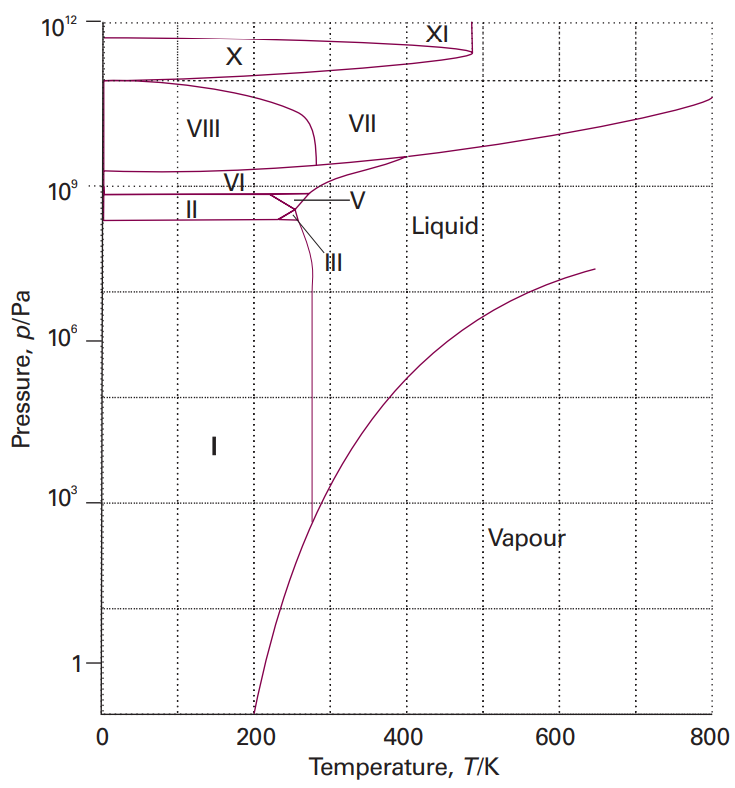
\includegraphics[width=0.8\textwidth]{images/phase-diagram.png}
  \caption{The phase diagram of water showing various phases of Ice, modified from (Atkins Physical Chemistry)}
  \label{fig:h2o-phasediag}
\end{figure}

\subsection{Reverse Monte Carlo}
If we want to explore a large configuration space in a manner which is computationally efficient, we must use some kind of stochastic algorithm, to drastically reduce the amount of unfavourable configurations that need to be computed. This is generally done using a Monte Carlo method, where random states are computed and then evaluated to reach an optimal state, using Markov Chains. Generally a Monte Carlo method employs some sort of randomisation step, an evaluation step, where some property of the configuration is evaluated and then a final averaging step, where the evaluations from various random configurations are collated to get a result which is more accurate than any of the individual parts. In our case, we will be doing these steps in reverse, going from experimentally gathered data, to try out various configurations and trying to find the optimal configuration.

We start with our experimentally acquired data, which we assign a ``certainty", a qualitative measure of how much we trust the data. The certainty will be used to allow a percentage of unfavourable configurations to be computed, so as to fully explore the configuration space. Next, we set up our initial environment, which is guess for the structure of the system. A diffraction pattern is then computed from this guess configuration. The system is then modified in small steps, using molecular dynamics, so as to produce ``adjacent" configurations. These configurations are then computed to produce a diffraction pattern. Both diffraction patterns (before the molecular dynamics and after) are then compared to the experimentally obtained data. If the new pattern is closer to the experimental data, it is accept, else it is rejected and the original pattern is accepted. Based on the certainty of the data, we accept unfavourable patterns as well, regardless of how close they were to the experimetal data. These steps are then repeated, with the new configuration (the accepted configuration or the unfavourable one if the certainty permits it) as the guess. In this way, we can explore the entire configuration space, while ignoring most of the unfavourable or energetically disallowed configurations.

RMC algorithms allow condensed matter physicists to explore the structure of a material with relative computational ease. The algorithm also produces quite accurate results, particularly for liquids and amorphous materials, where it is one of the only computational tools at the disposal. Additionally, due to its stochastic nature, the algorithm is also useful for computing the structures of inherently disordered materials, like Ice VII.

\begin{figure}
  \centering
  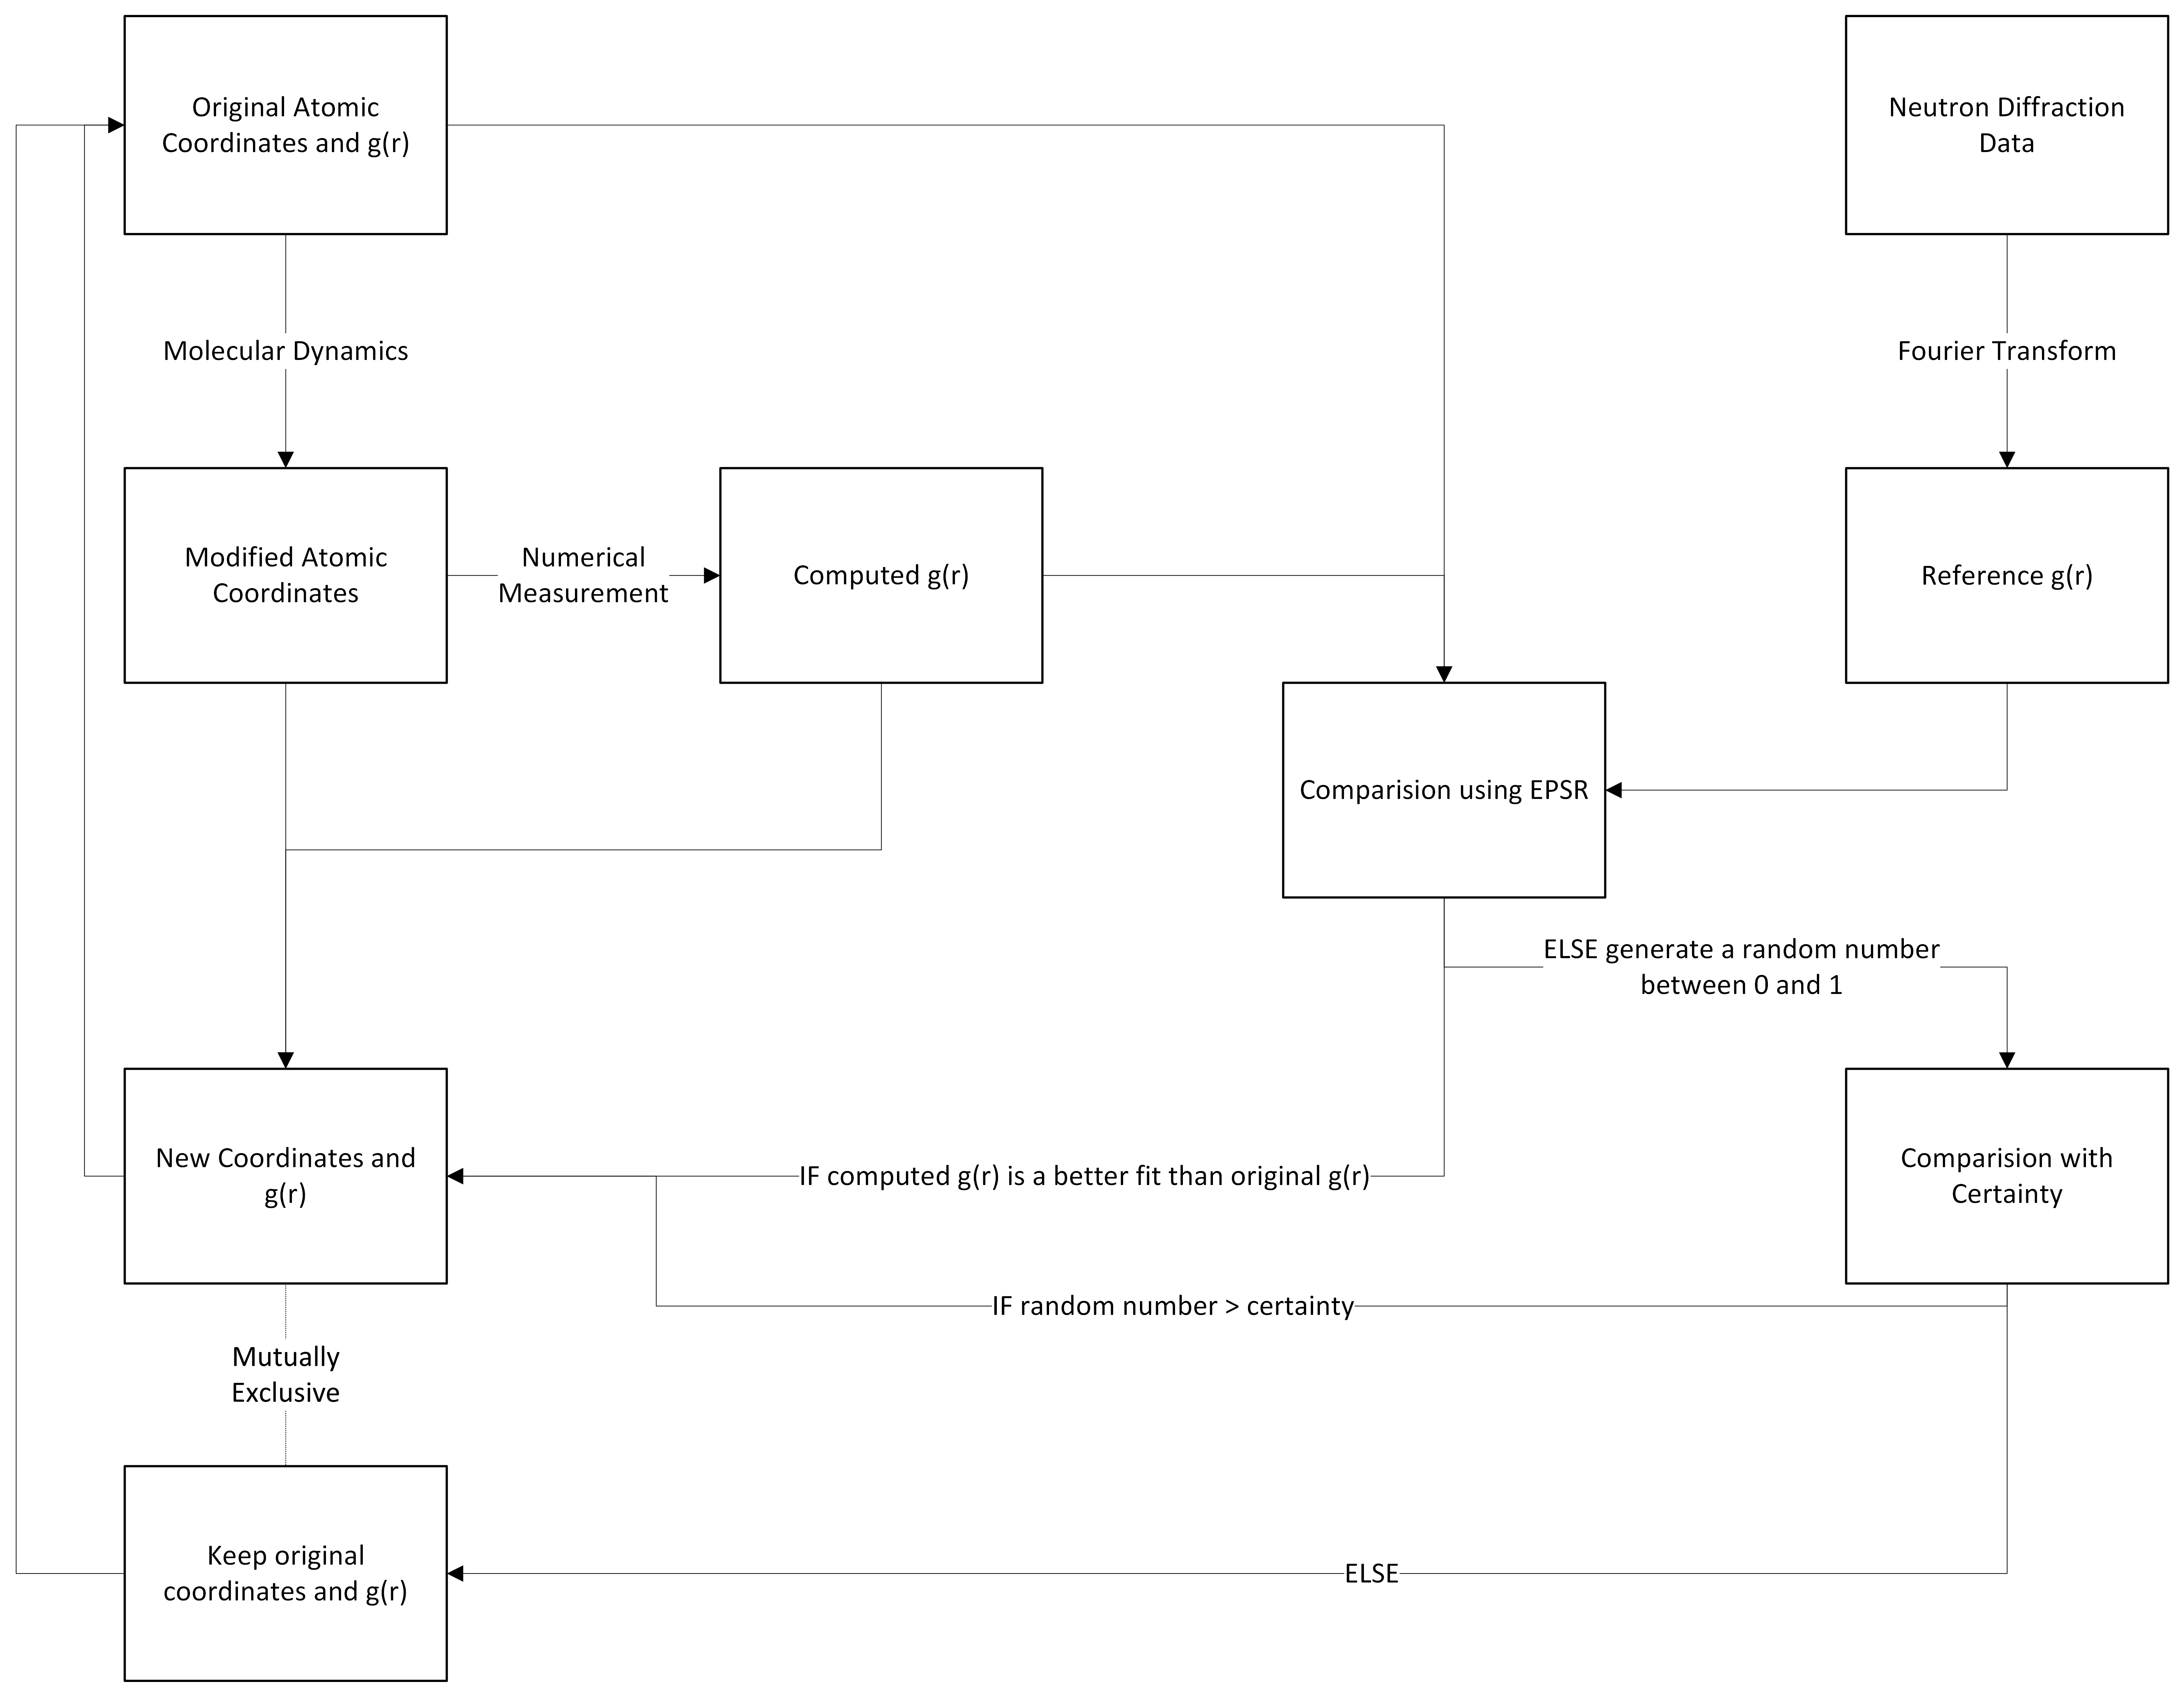
\includegraphics[width=\textwidth]{images/RMCWorkflow.png}
  \caption{The workflow of a Reverse Monte Carlo simulation with EPSR, created using Microsoft Visio}
  \label{fig:rmc-workflow}
\end{figure}

\subsection{Condensed Matter Theory}
\subsubsection{Neutron Diffraction}
Neutron diffraction is a technique used to determine the structure of a material. It is similar to X-ray diffraction, but instead of using X-rays, it uses neutrons. Neutrons are used instead of X-rays since they have a higher scattering cross section, which allows them to penetrate deeper into the material. This allows us to use neutron diffraction to determine the structure of materials which are opaque to X-rays. Neutron diffraction is also useful for determining the positions of light atoms, such as hydrogen, which have a low scattering cross section for X-rays. Additionally, because neutrons are uncharged, they do not interact with the electrons in the material, which allows us to determine the positions of the nuclei of the atoms in the material, without having to account for the electrons. Neutrons are also heavy particles, which means that a neutron beam will have little intensity drop off even for large scattering angles. This allows us to use neutron diffraction to determine the structure of materials with large unit cells and with much higher accuracy than X-ray diffraction.
\subsubsection{Radial Distribution Function}
The radial distribution function (RDF) is a measure of the probability of finding an atom at a distance $r$ from another atom. It is defined as the ratio of the probability of finding an atom at a distance $r$ from another atom, to the probability of finding an atom at the same distance in an ideal gas. The RDF is a useful measure of the structure of a material, since it allows us to see how atoms are distributed around each other. By investigating the RDF of various atom combinations, we can see how the structure of the material changes with different phases. This allows us to quantitatively compare the structure of Ice VII with liquid water and also with other phases of Ice, such as Ice VIII or Ice X.

The RDF can be determined experimentally from Neutron diffraction data. The diffraction pattern is Fourier transformed to get the RDF in a particular direction. The RDF can also be computed from simulations, by counting the number of atoms at a given distance from another atom, and then normalising it by the number of atoms in the system and the volume of the system. As such, comparing the total RDF in a particular direction, shown as $g(r)$ from here on in, between the simulation and the experimental data allows us to see how well the simulation matches the experimental data.
\section{Methodology}
\subsection{Software}
Since the project involves simulations, the choice of software used will be important. The various choices made in the project are listed below, as well as the reasoning behind them.
\subsubsection{Dissolve}
For the purposes of this project, we shall be using Dissolve, a computational package which allows us to run reverse monte carlo simulators at scale, with relative computational efficiency. Dissolve also has a graphical user interface which allows easier input of data, and makes the learning curve for the software less steep. This allows scientists not traditionally trained in computational methods to also use dissolve with relative ease.
\subsubsection{Hydrogen Bond Network Measurement}
To compare the results between different bond networks in Ice VII and Water, we wrote a program in C. Initially, the program would take in positions of atoms from the simulation, and then use pathfinding algorithms to locate sequentially closer atoms. These atoms would then be checked to see if they form loops. While successful, this method was computationally expensive and unoptimised. Thus for computational efficiency, a linear algebra and graph theory based method was used instead.

In the linear algebra and graph theory based method, we create a $n \times n$ matrix, where $n$ is the number of atoms in the system. Every element on this matrix $A_{ij}$ represents the distance from the atom at index i to the atom at index j. This matrix is then reduced to a boolean matrix such that if the distance is less than a given threshold (the minimum threshold for the formation of hydrogen bonds), we assign it a value of ``1" or ``true" and otherwise it takes the value ``0" or ``false". Now we can use elementary graph theory to detect loops, considering the matrix to be a representation of a undirected graph with $n$ nodes, with each element in the matrix storing whether or not the node is connected to another node.

The advantage of using the linear algebra and graph theory based method is that we can parallelise the computation, which allows us to take advantage of scale and compute the number of loops for a larger number of configurations, or for larger configurations. OpenMP is used to implement parallelisation in the code used in the project, however similar packages can be used for other languages.
\section{Results}
\begin{figure}[H]
  \centering
  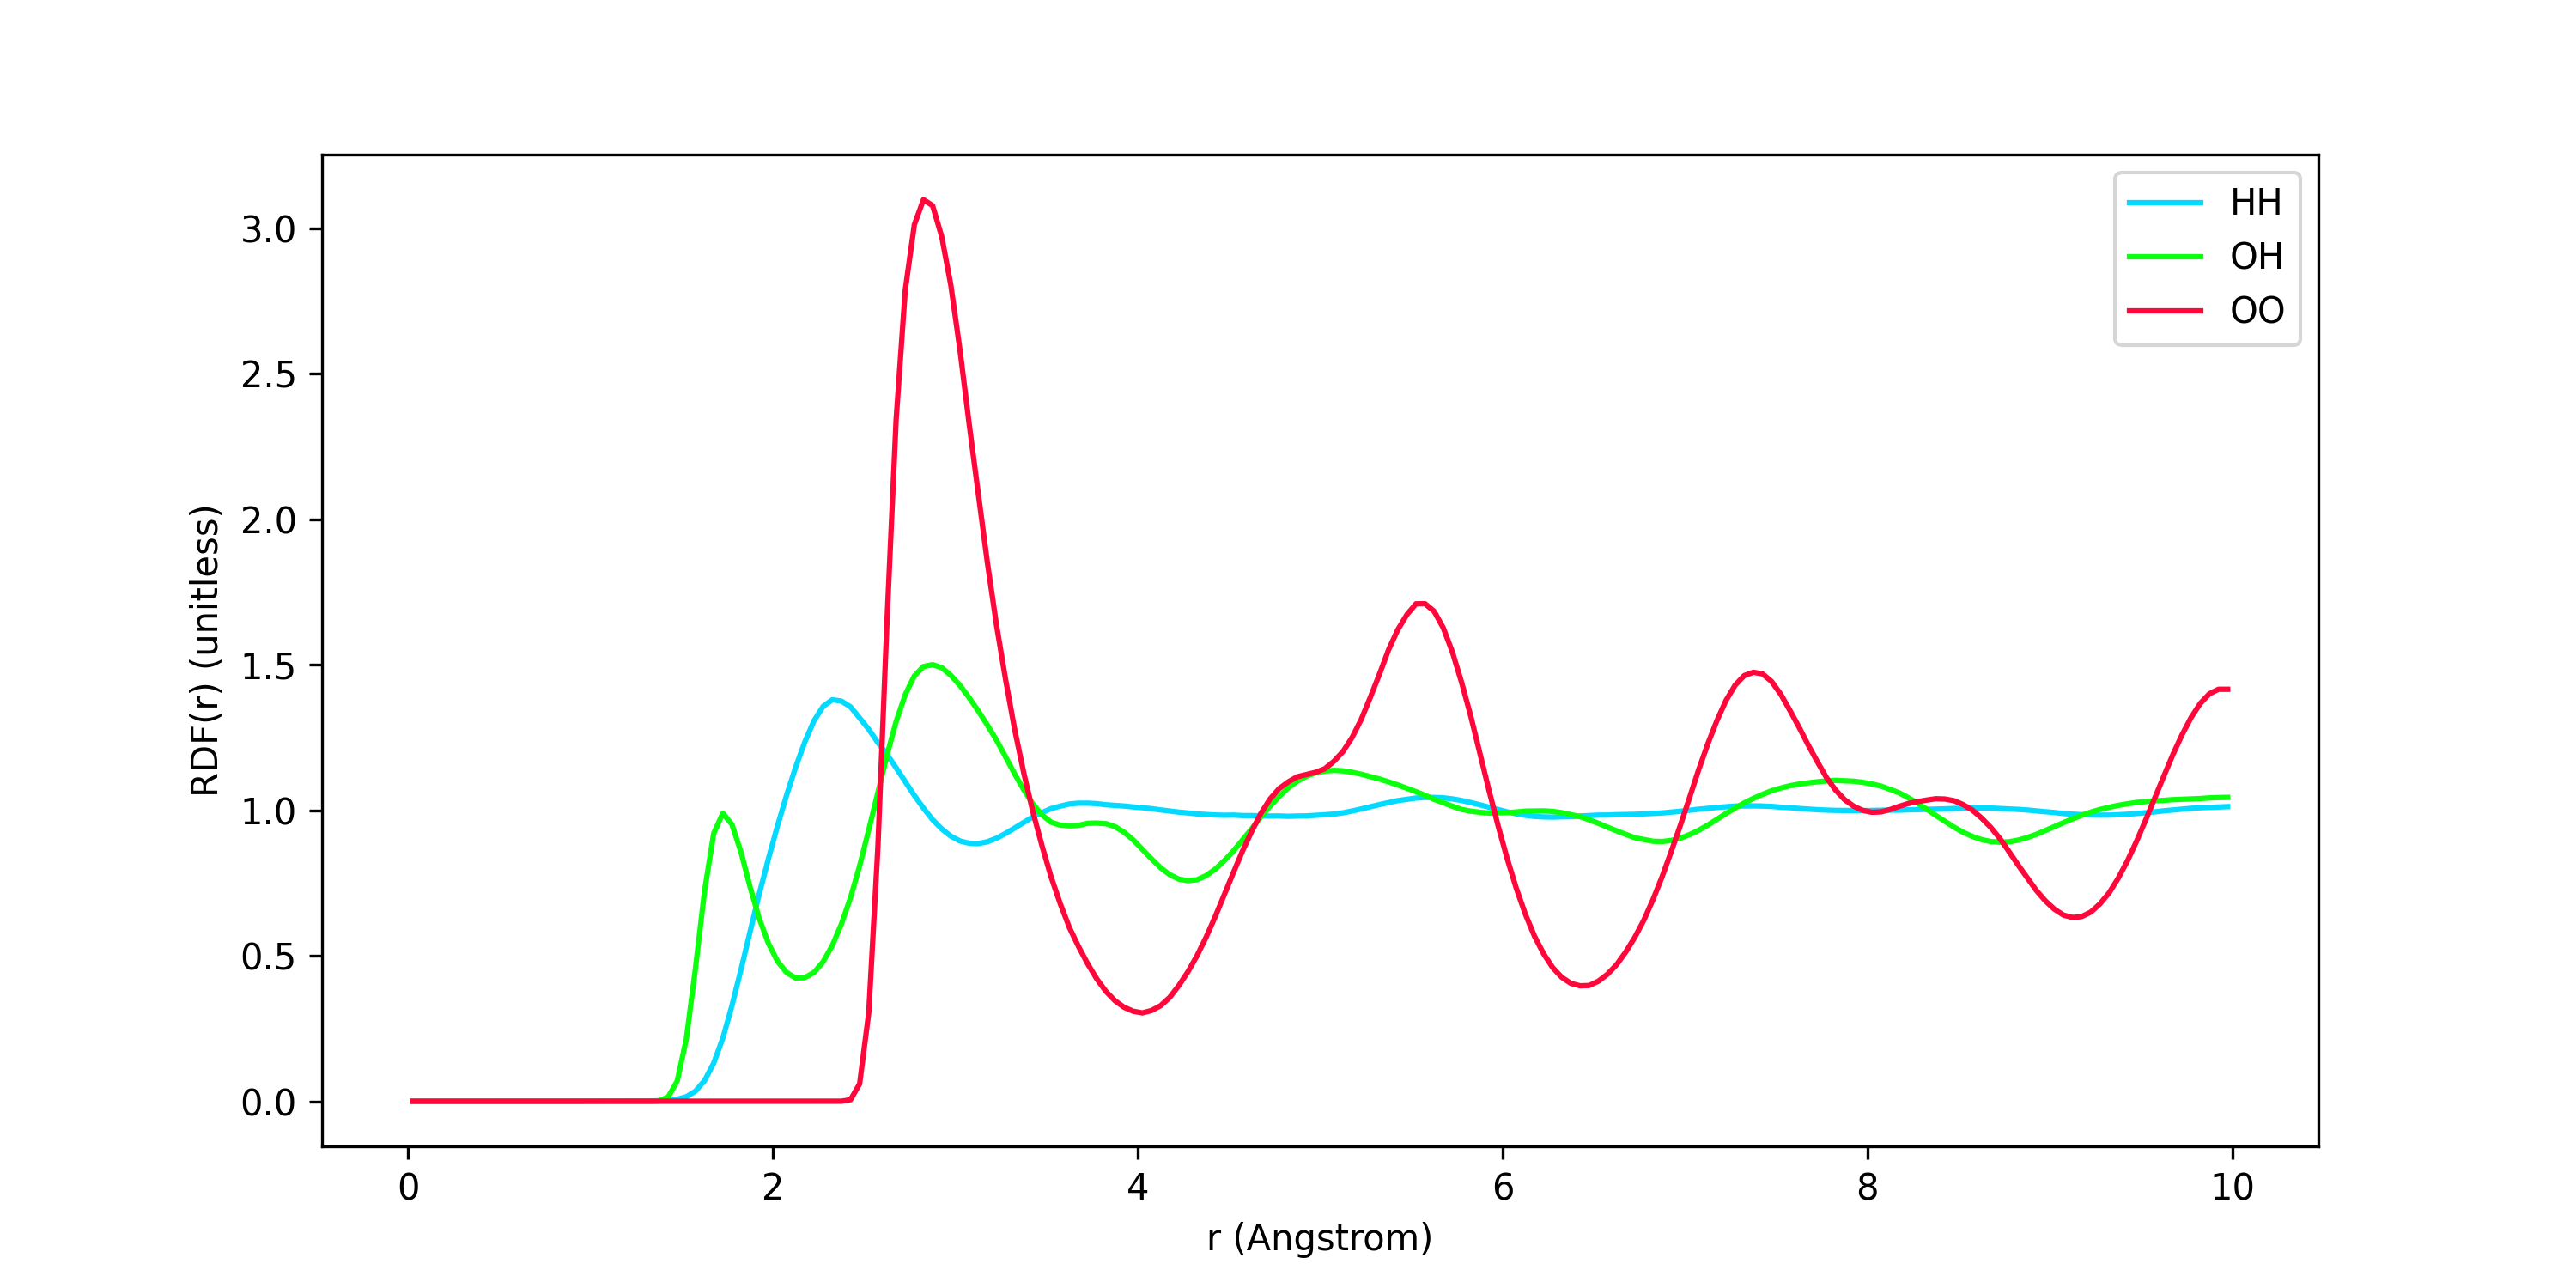
\includegraphics[width=\textwidth]{images/RDF.png}
  \caption{The radial distribution functions of various atom combinations}
  \label{fig:rdf}
\end{figure}
\begin{figure}[H]
  \centering
  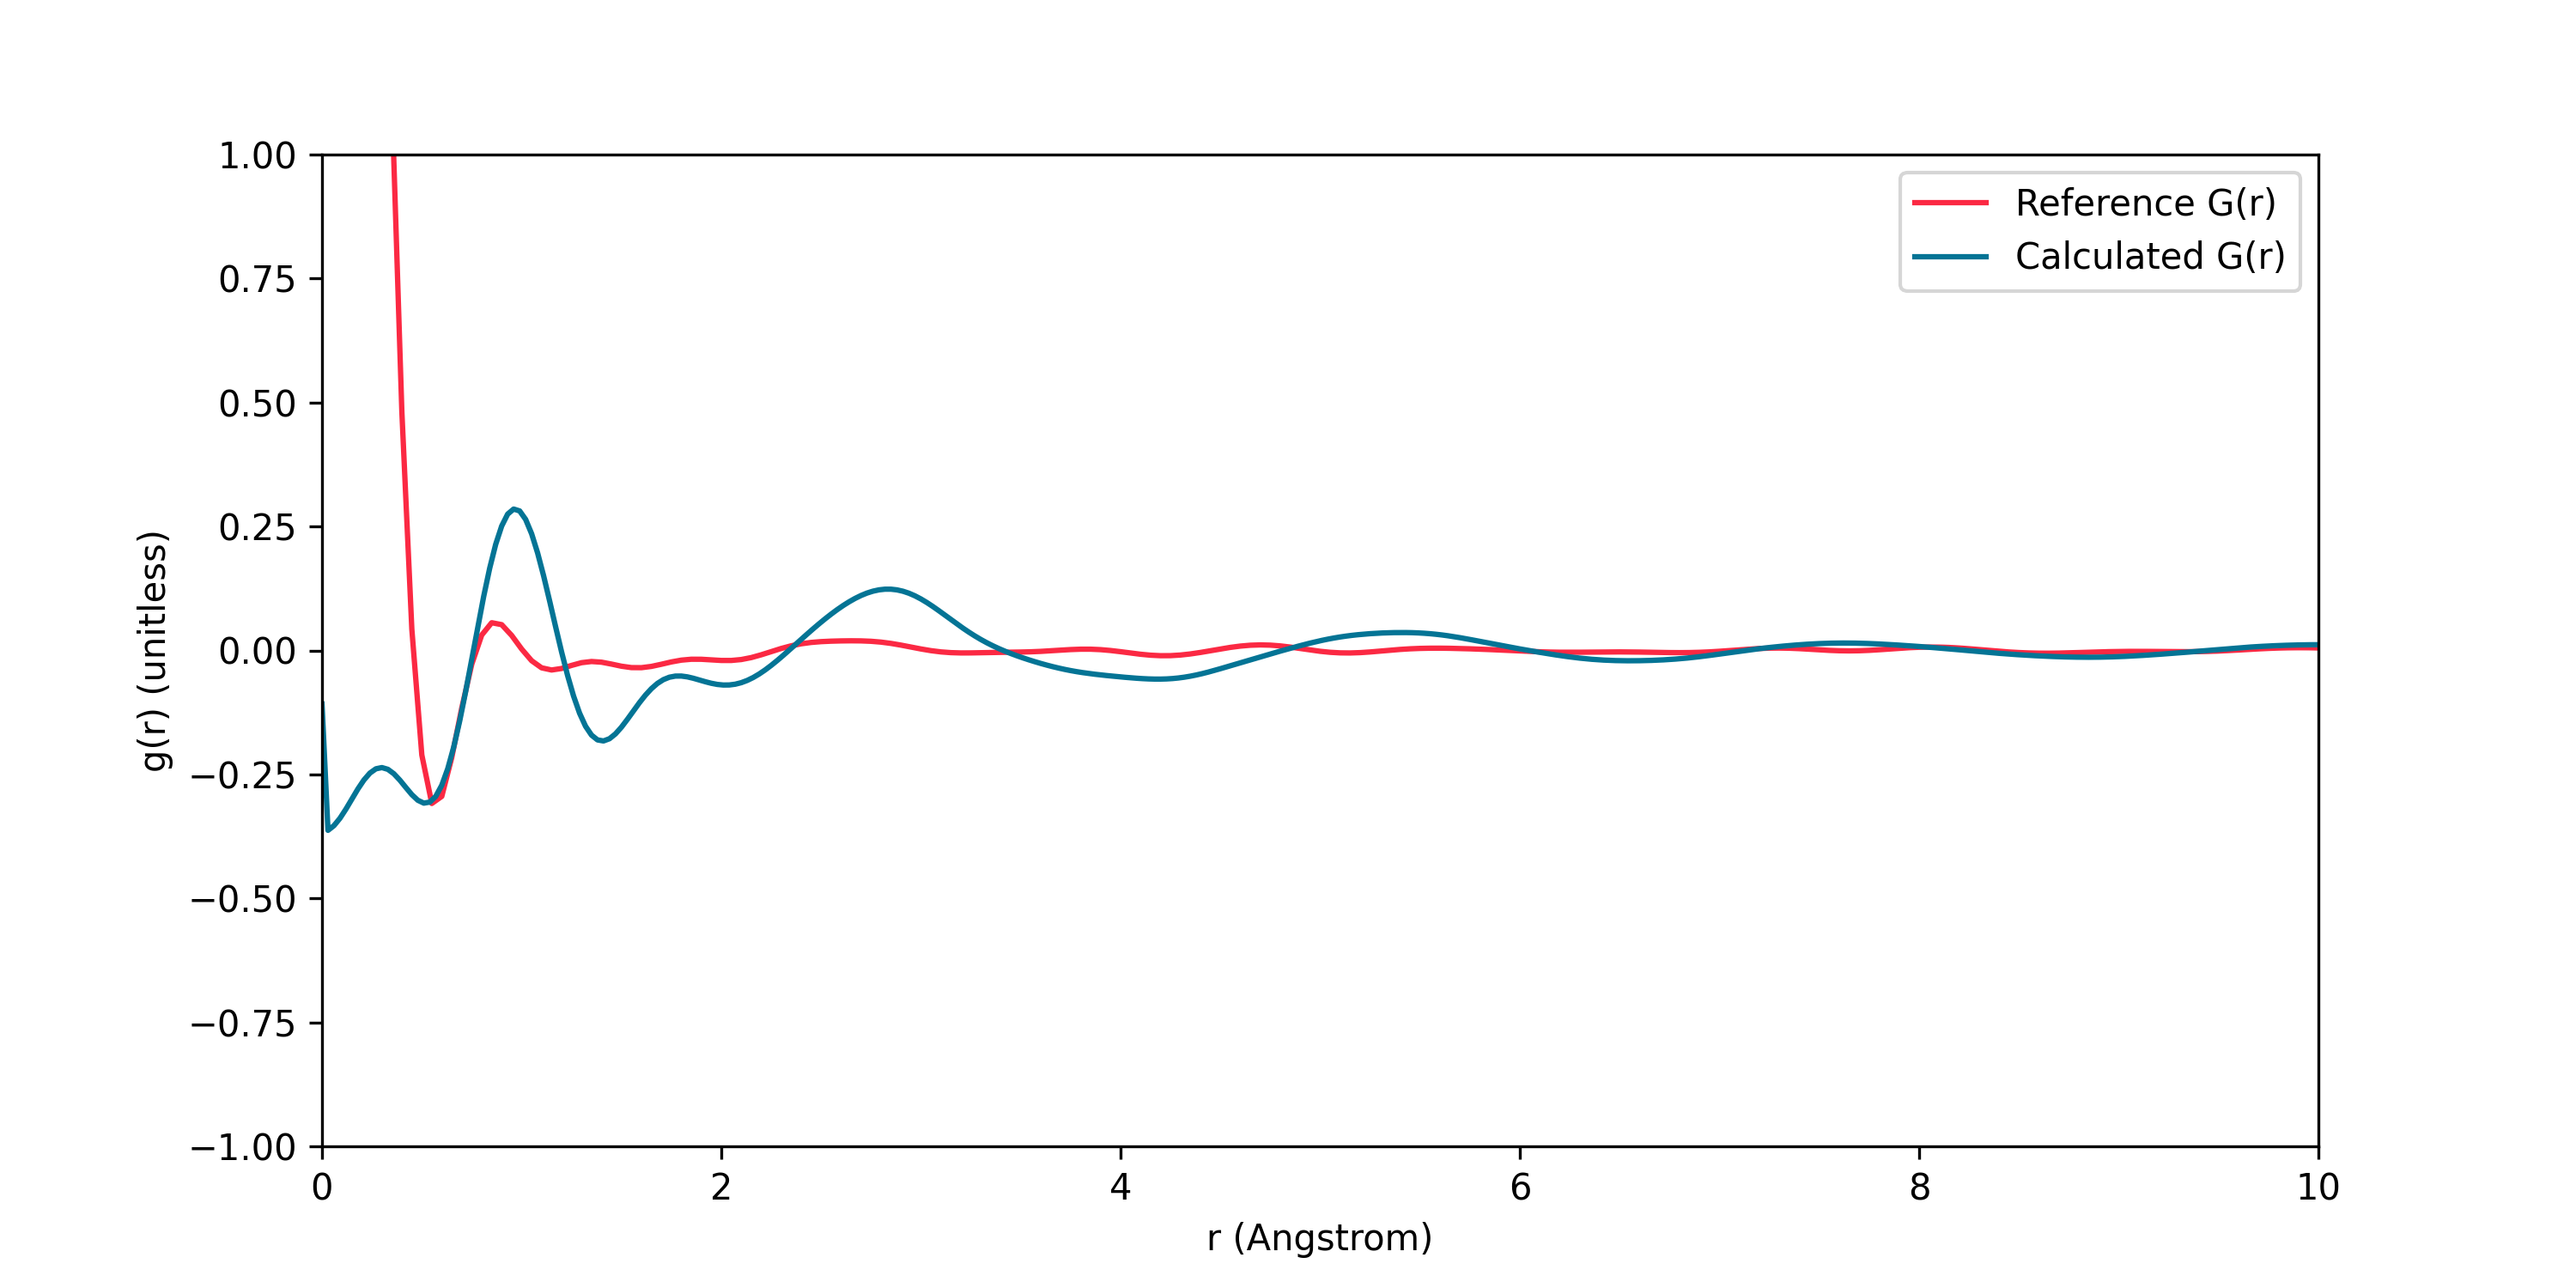
\includegraphics[width=\textwidth]{images/GR.png}
  \caption{The G(r) distribution calculated by Dissolve, compared to the G(r) from the Fourier Transformation of the Reference Data}
  \label{fig:gr}
\end{figure}
\begin{figure}[H]
  \centering
  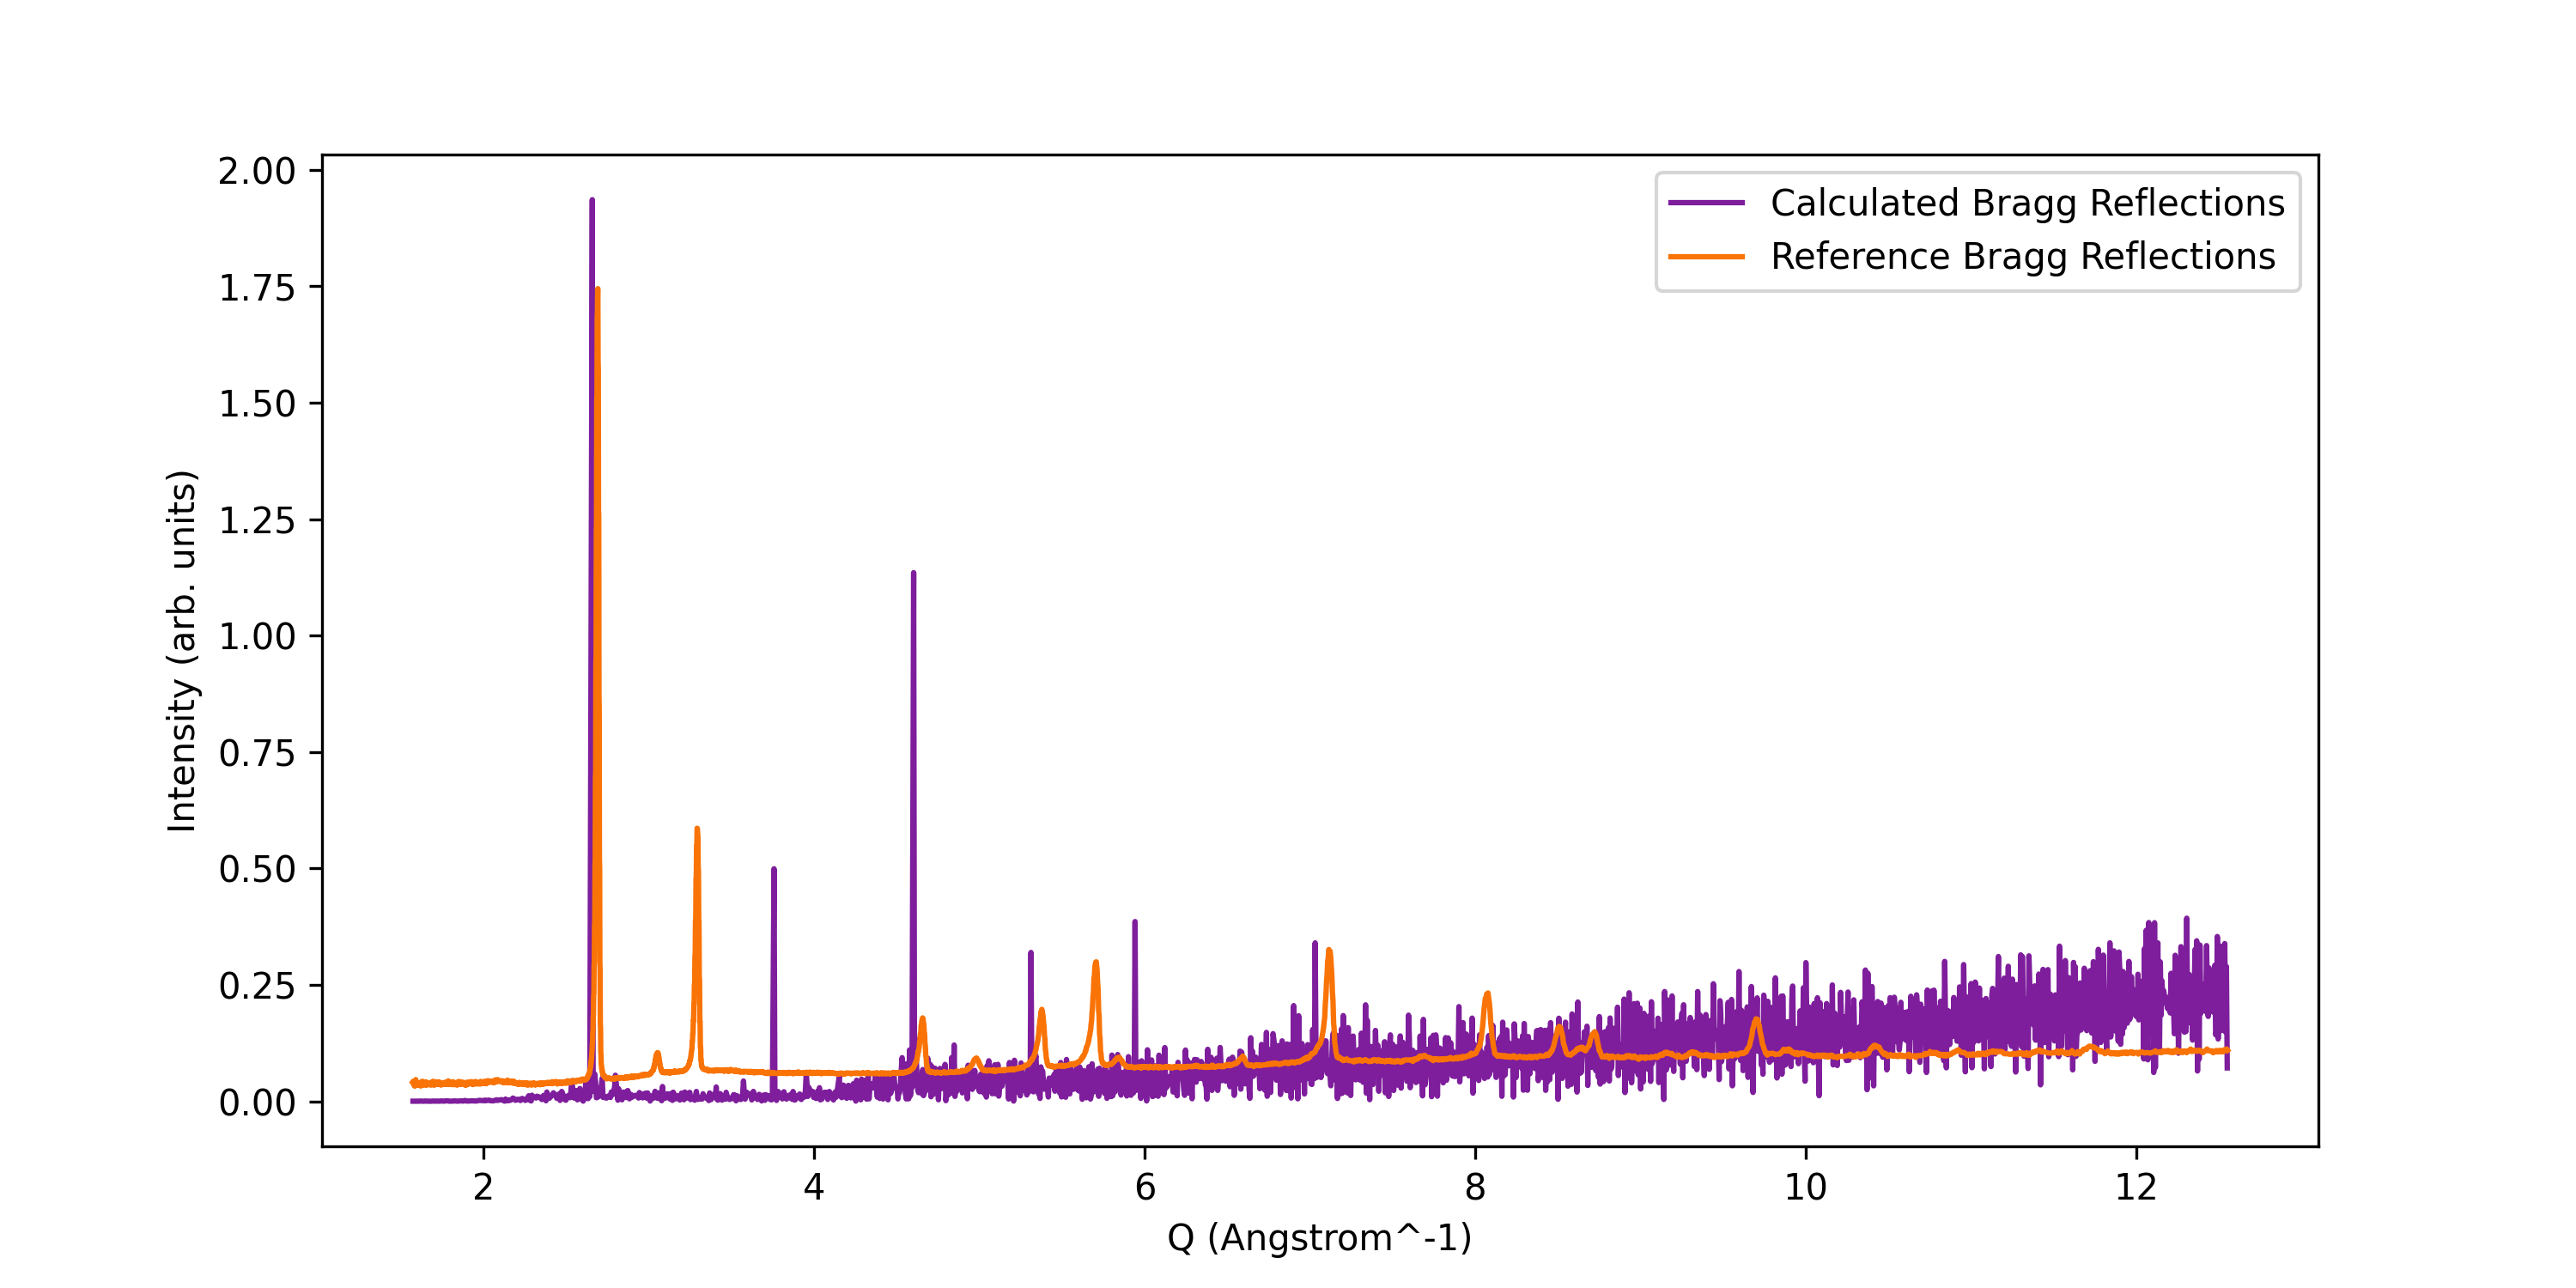
\includegraphics[width=\textwidth]{images/Bragg.png}
  \caption{The Bragg distribution calculated by Dissolve, compared to the experimental Bragg distribution}
  \label{fig:bragg}
\end{figure}
\begin{figure}[H]
  \centering
  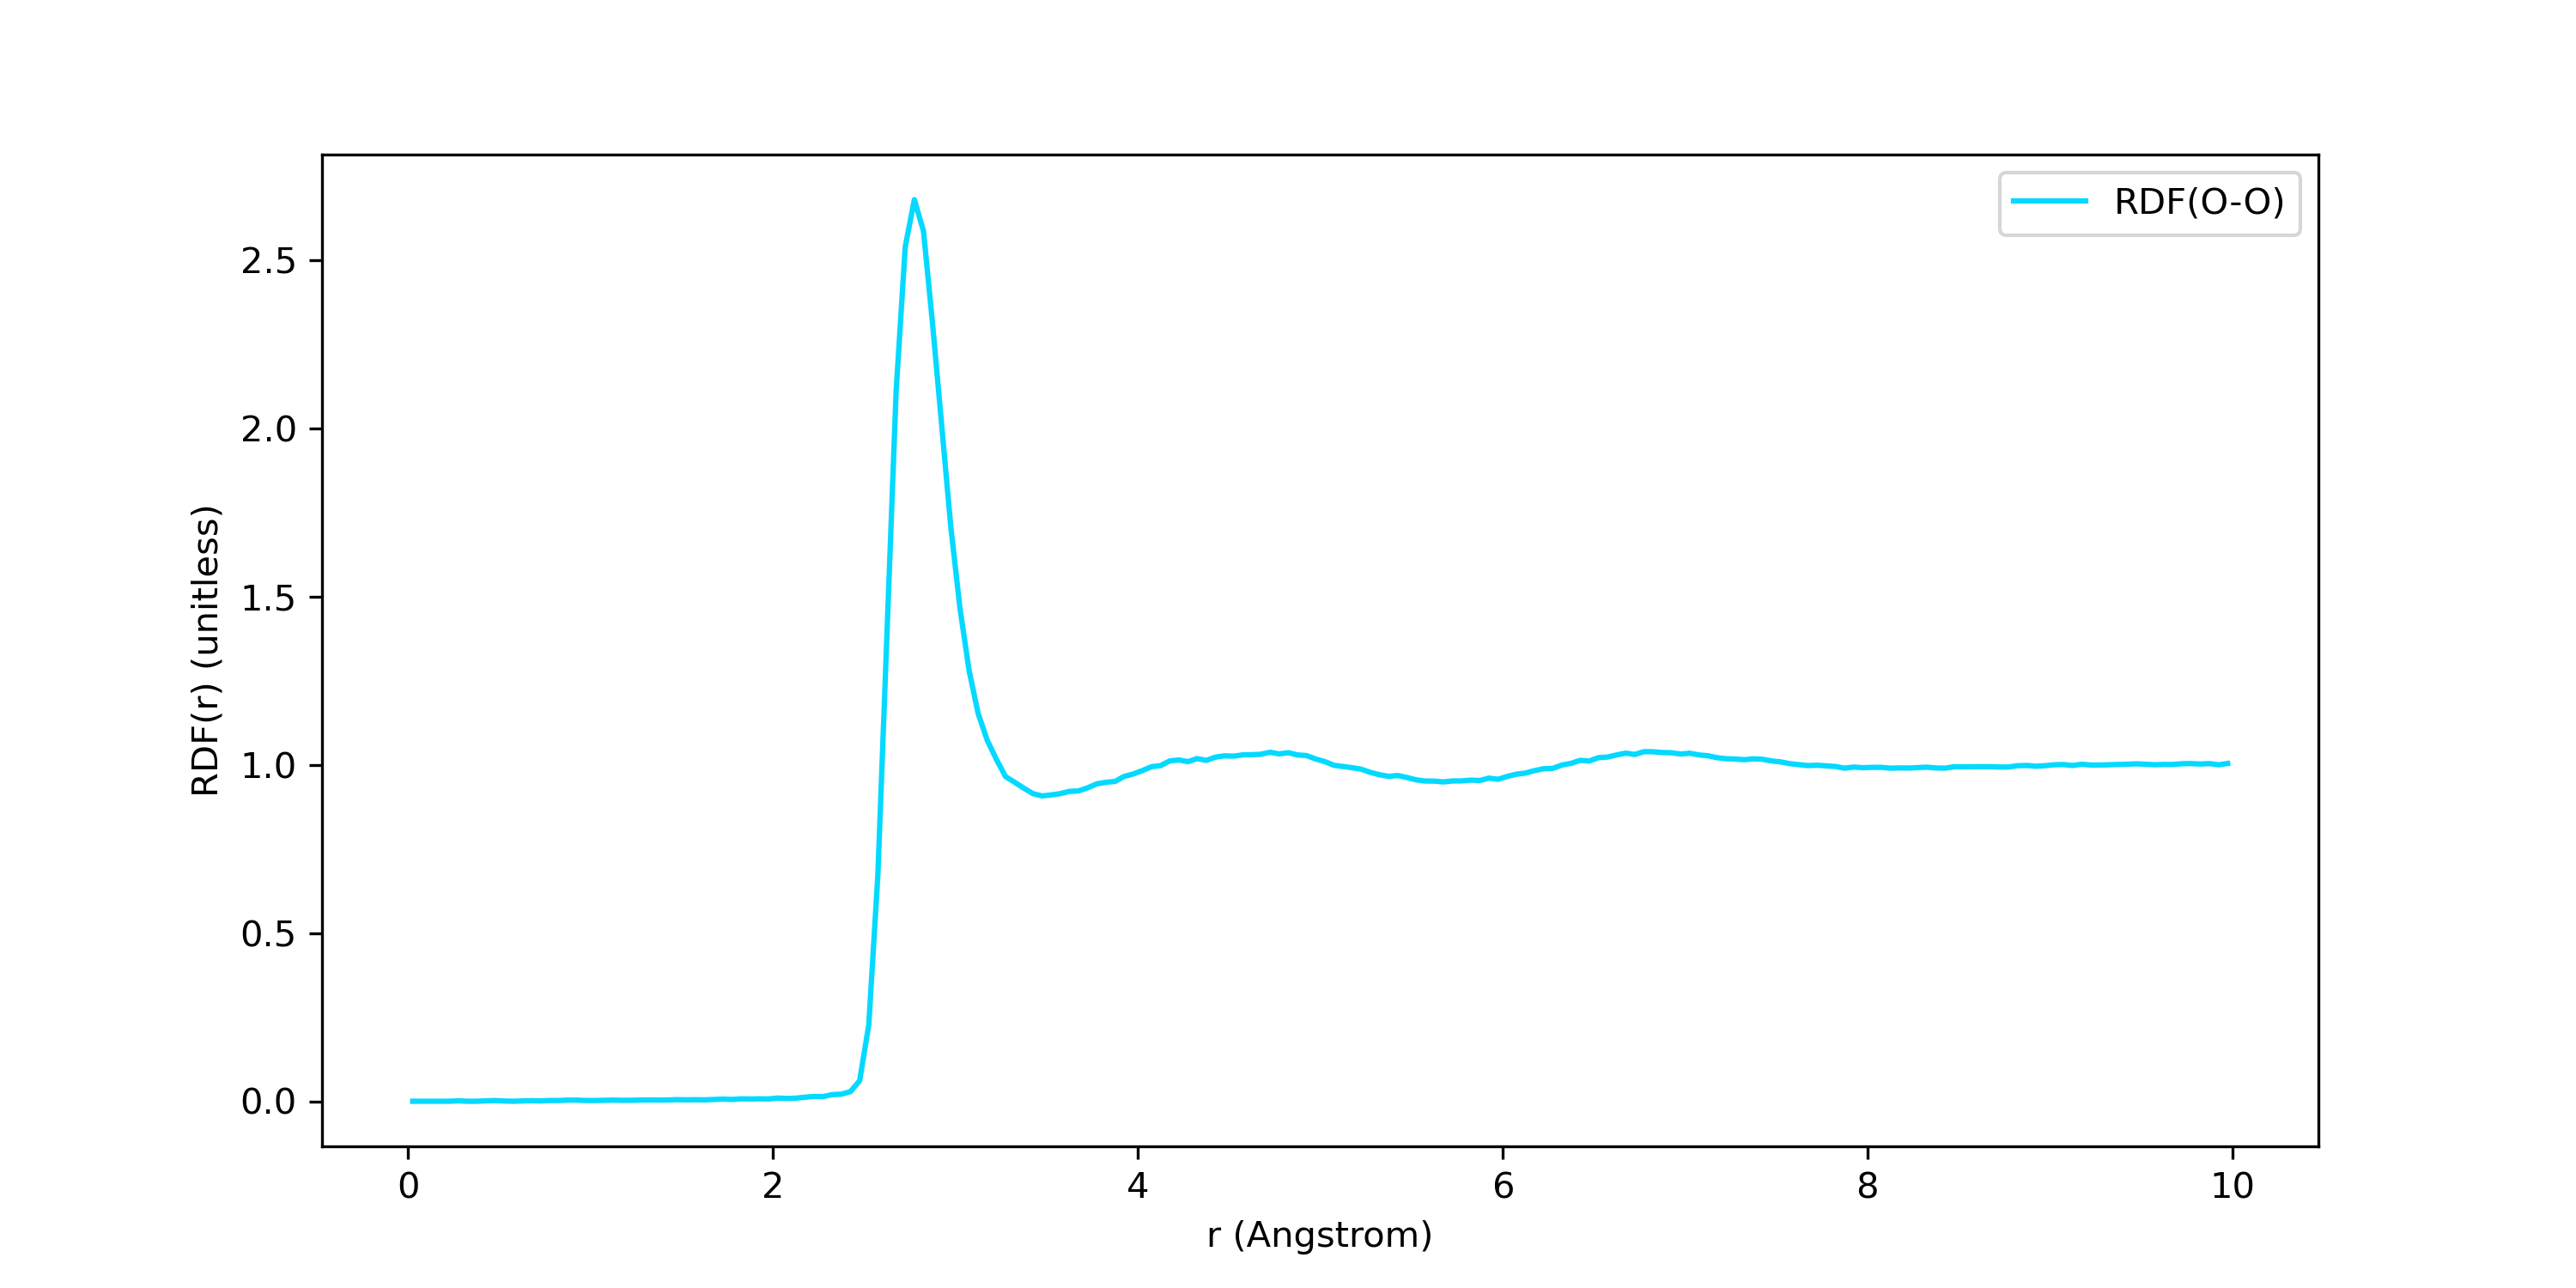
\includegraphics[width=\textwidth]{images/RDF-liquid.png}
  \caption{The Bragg distribution calculated by Dissolve, compared to the experimental Bragg distribution}
  \label{fig:rdf-liquid}
\end{figure}
\begin{figure}[H]
  \centering
  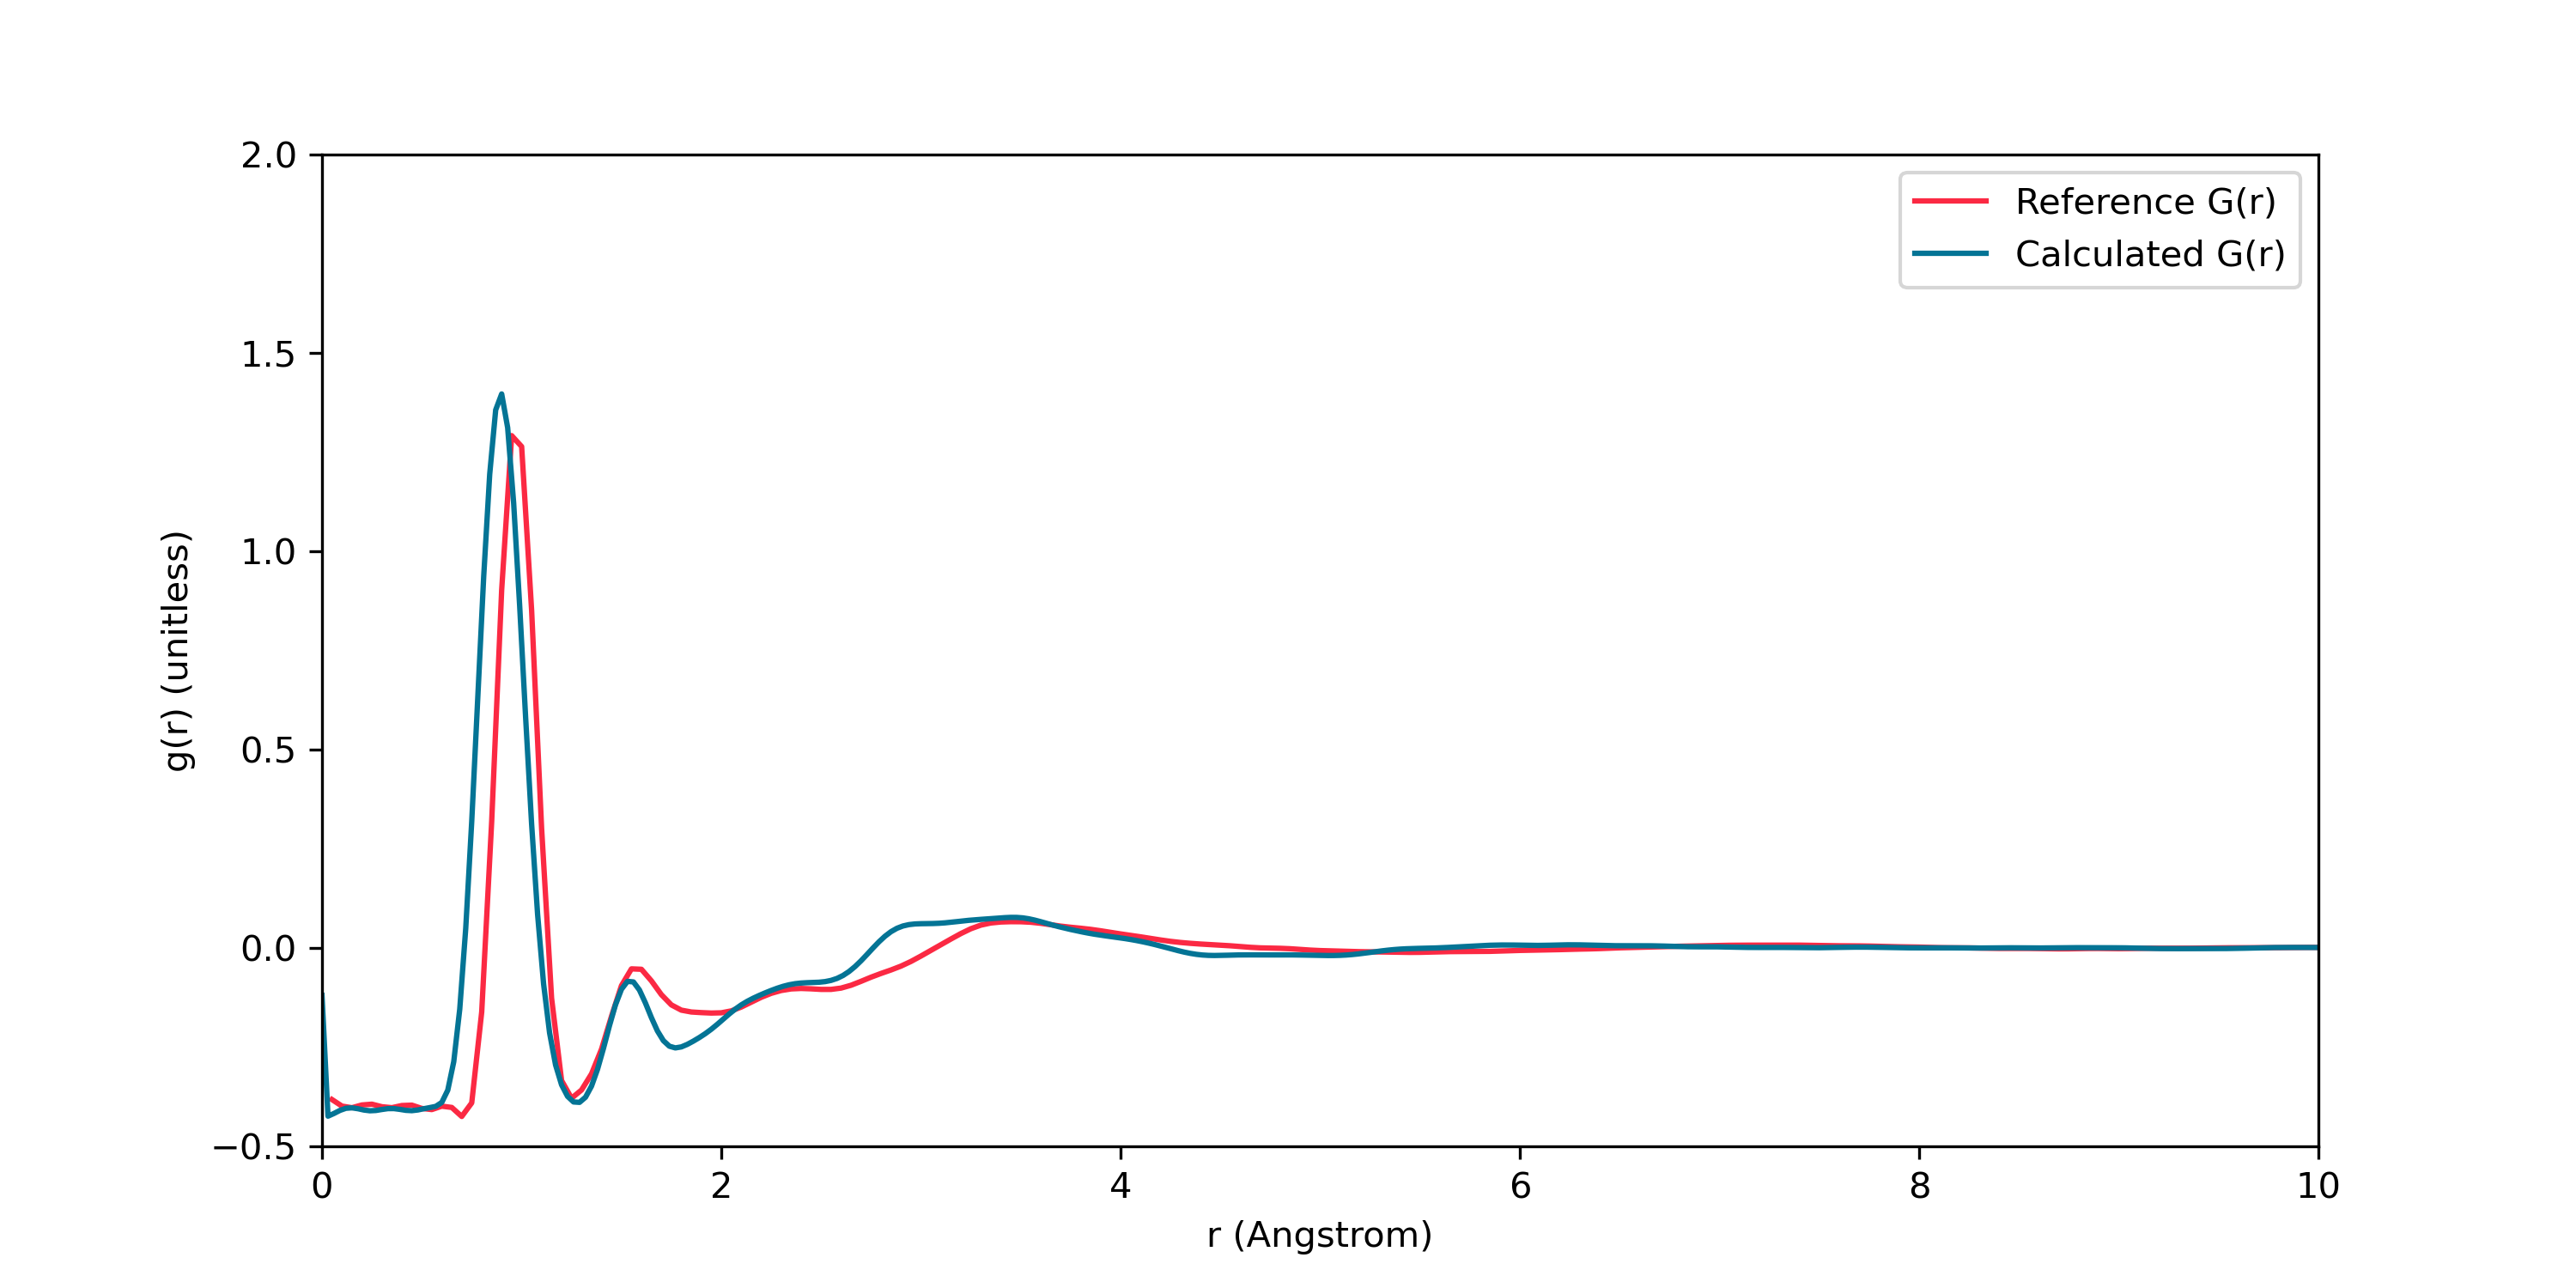
\includegraphics[width=\textwidth]{images/GR-liquid.png}
  \caption{The Bragg distribution calculated by Dissolve, compared to the experimental Bragg distribution}
  \label{fig:gr-liquid}
\end{figure}
\section{Discussion}
\subsection{Comparison with Past Work}
\subsection{Limitations}
\subsection{Impact and Further Research}
A long time goal of condensed matter physics has been to be able to determine the structure of a crystal based solely on its chemical composition and physical conditions. Currently there is no way to do this purely analytically, and the only way to determine the structure of a crystal is through experimental methods. However, the advent of computational methods, such as the reverse monte carlo methods used by us in this project, have created a new range of ``semi-empirical'' tools, which allow us to bridge the gap between theory and experiment. They allow us to use theoretical models for a material, and then add disorder to it in a way that is consistent with experimental data, allowing us to better model the material as it exists in reality. While of course this is a far cry from being able to determine the structure of a material purely analytically, it is a step in the right direction, and allows us to better understand the structure of materials, and how they change with different conditions.

Another interesting avenue of research would be to combine reverse monte carlo methods, with other tools such as density functional theory. A disordered structure generated by a reverse monte carlo method could be used as the input for a density functional theory calculation, which could then be used to refine the structure and deduce the physical properties of the material. The added disorder would enable the density functional theory calculations to model properties that it would otherwise be unable to, such as certain surface effects or even the effect of impurities. On a similar note, RMC methods could be combined with chemical dynamics simulations to better simulate the kinetics of chemical reactions in a solvent, since RMC methods are effective at modelling liquids.
\section{Conclusion}
\section{Appendices}
\subsection{Acknowledgements}
I would like to thank Dr. Ciprian Pruteanu for his guidance and support throughout the project. I would also like to thank the School of Physics and Astronomy at the University of Edinburgh for providing me with the opportunity to work on this project. I would also like to thank my community of friends and mentors, particularly Abdul Malik ibn Marwan and Jorge Mario Bergoglio for their spiritual support and guidance. Finally, since scientific knowledge is a social product, I would like to thank all the scientists who have worked on this topic before me, and whose work has made this project possible.
\subsection{Code}
\subsection{References}
\end{document}